\documentclass[12pt,a4paper]{article}
\usepackage[utf8]{inputenc}
\usepackage[T1]{fontenc}
\usepackage[margin = 0.5in, top = 1in]{geometry}
\usepackage{fancyhdr}
\usepackage{physics}
\usepackage{amssymb}
\usepackage{graphicx}
\usepackage{hyperref}
\usepackage{float}
\usepackage{subfig}
\usepackage{verbatim}
\usepackage{svg}
\usepackage{textgreek}
\usepackage{tikz}
\usetikzlibrary{bayesnet}
\usetikzlibrary{matrix}
\usepackage[doublespacing]{setspace}
\usepackage[toc,page]{appendix}
\restylefloat{table}
\pagestyle{fancy}
\fancyhf{}
\newcommand{\Ti}{Project nr 2}
\newcommand{\Author}{Mateusz Kapusta}
\newcommand{\dane}{\mathcal{D}}
\newcommand{\Title}{Project nr 2}
\tikzset{ 
    table/.style={
        matrix of nodes,
        row sep=-\pgflinewidth,
        column sep=-\pgflinewidth,
        nodes={
            rectangle,
            draw=black,
            align=center
        },
        minimum height=1.5em,
        text depth=0.5ex,
        text height=2ex,
        nodes in empty cells,
%%
        every even row/.style={
            nodes={fill=gray!20}
        },
        column 1/.style={
            nodes={text width=1em,font=\bfseries}
        },
        row 1/.style={
            nodes={
                fill=black,
                text=white,
                font=\bfseries
            }
        }
    }
}
\title{\huge \bf \Title\\ Gibbs sampling}
\author{Mateusz Kapusta}
\DeclareRobustCommand{\bbone}{\text{\usefont{U}{bbold}{m}{n}1}}
\DeclareMathOperator{\EX}{\mathbb{E}}% expected value
\rhead{\it \Ti}
\lhead{\Author}
\begin{document}
\maketitle
\section{Rain BBN}
\begin{figure}[H]\label{var_enc}
    \centering
    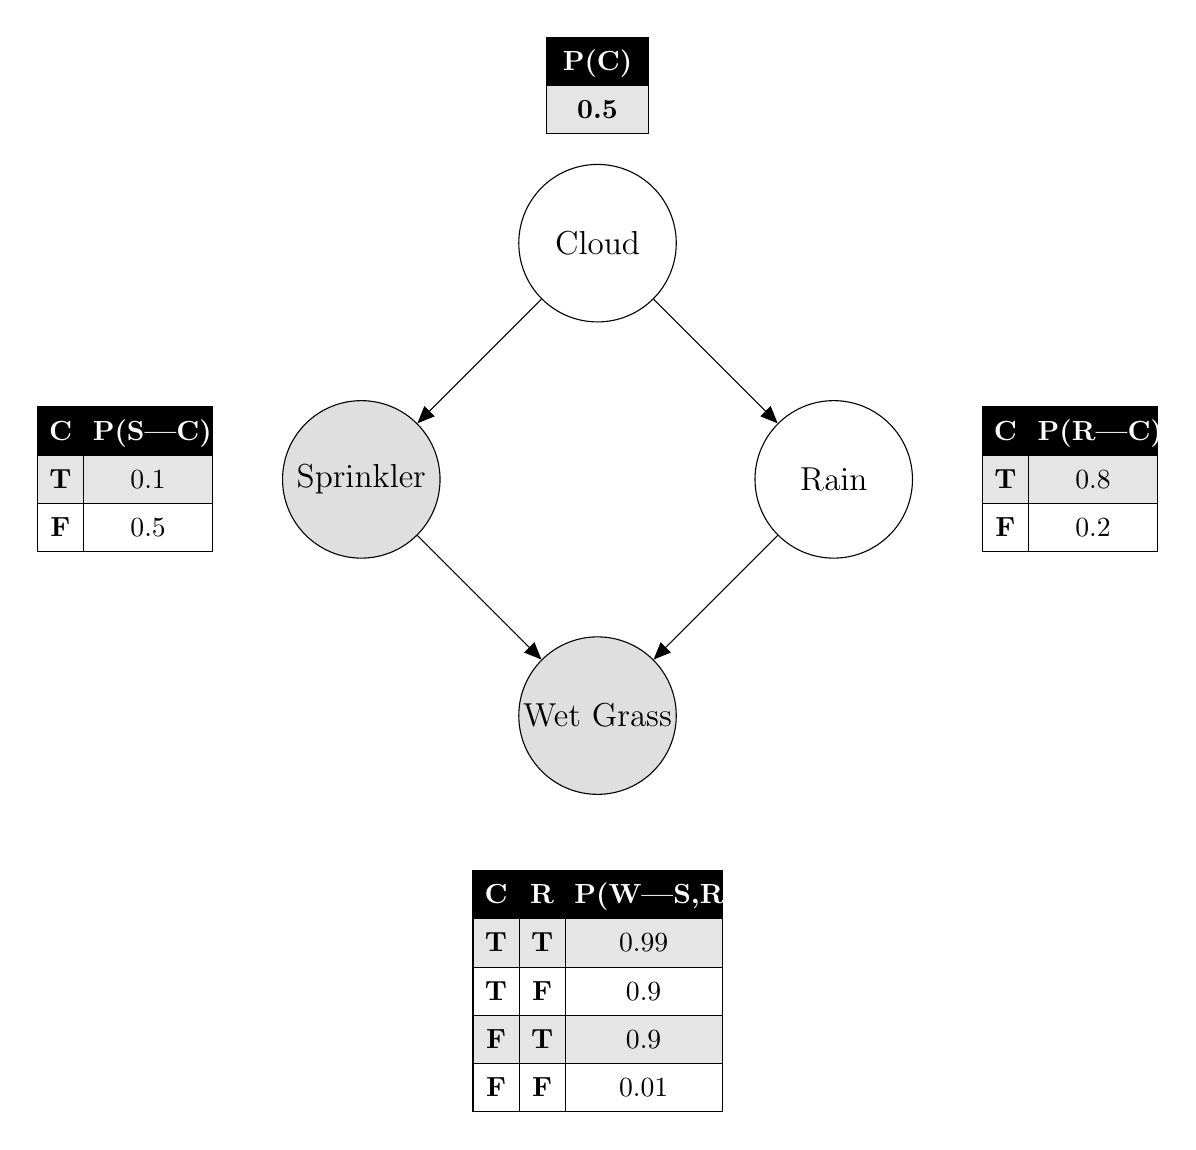
\begin{tikzpicture}
        \node[latent,minimum size=2cm] (cloud) at (0,0) {\large Cloud\par\par\par};
        \node[latent,minimum size=2cm] (rain) at (3,-3) {\large Rain   };
        \node[obs,minimum size=2cm] (sprinkler) at (-3,-3) {\large Sprinkler};
        \node[obs,minimum size=2cm] (grass) at (0,-6) {\large Wet Grass};
        \path[draw, ->] (cloud) edge (rain);
        \path[draw,->] (cloud) edge (sprinkler);
        \path[draw,->] (sprinkler) edge (grass);
        \path[draw,->] (rain) edge (grass);

        \matrix (sprink_matrix) [table,text width=4em] at (-6,-3)
        {
        C & P(S|C)\\
        T   & 0.1\\
        F   & 0.5\\
        };

        \matrix (rain_matrix) [table,text width=4em] at (6,-3)
        {
        C & P(R|C)\\
        T   & 0.8\\
        F   & 0.2\\
        };

        \matrix (grass_matrix) [table,text width=5em,column 2/.style={
            nodes={text width=1em,font=\bfseries}
        },] at (0,-9.5)
        {
        C & R &  P(W|S,R)\\
        T & T  & 0.99\\
        T & F  & 0.9\\
        F & T  & 0.9\\
        F & F  & 0.01\\
        };
        \matrix (cloud_matrix) [table,text width=4em,column 1/.style={
            nodes={text width=3em,font=\bfseries}
        },] at (0,2)
        {
        P(C)\\
        0.5\\
        };
    \end{tikzpicture}
    \caption{Bayesian diagram for rain network}\label{Rain}
\end{figure}
\hspace{1cm}\par Let's conisder Bayesian Belif network depicted at \ref{Rain}. Each of the varibles can be either True or False. Conditional dependence between them in encoded in the matrix next 
to each of the nodes. Right now let's do not think about which varibles are observed and try to dervie formula for propability of one node with respect to other varibles which remain constant
\begin{enumerate}
    \item {\Large \textbf{$P(C=T|R=T,S=T,W=T)$}}\\
    We can decompose local propability distribution to 
    \begin{equation*}
        P(C=T|R=T,S=T,W=T)\propto P(S=T|C=T)P(R=T|C=T)=0.1\cdot0.8=0.08
    \end{equation*}
    In order to find true propability we need to compute renormalazing constant
    \begin{equation*}
        P(C=F|R=T,S=T,W=T)\propto P(S=T|C=F)P(R=T|C=F)=0.5\cdot0.2=0.10
    \end{equation*}.
    After renomalization
    \begin{equation*}
        P(C=T|R=T,S=T,W=T)=\frac{0.08}{0.08+0.1}\approx0.44
    \end{equation*}

    \item{\Large \textbf{$P(C=T|R=F,S=T,W=T)$}}\\
    As before
    \begin{equation*}
        P(C=T|R=F,S=T,W=T)\propto P(S=T|C=T)P(R=F|C=T)=0.1\cdot0.2=0.02
    \end{equation*}
    In order to find true propability we need to compute renormalazing constant
    \begin{equation*}
        P(C=F|R=F,S=T,W=T)\propto P(S=T|C=F)P(R=F|C=F)=0.5\cdot0.8=0.4
    \end{equation*}.
    After renomalization
    \begin{equation*}
        P(C=T|R=F,S=T,W=T)=\frac{0.02}{0.02+0.4}\approx0.047
    \end{equation*}

    \item {\Large \textbf{$P(R=T|C=T,S=T,W=T)$}} \\
    As before
    \begin{equation*}
        P(R=T|C=T,S=T,W=T)\propto P(W=T|R=T,S=T)P(R=T|C=T)=0.99\cdot0.8=0.792
    \end{equation*}
    In order to find true propability we need to compute renormalazing constant
    \begin{equation*}
        P(R=F|C=T,S=T,W=T)\propto P(W=T|R=F,S=T)P(R=F|C=T)=0.9\cdot0.2=0.18
    \end{equation*}.
    After renomalization
    \begin{equation*}
        P(R=T|C=T,S=T,W=T)=\frac{0.792}{0.18+0.792}\approx0.81
    \end{equation*}

    \item {\Large \textbf{$P(R=T|C=F,S=T,W=T)$}}\\
    As before
    \begin{equation*}
        P(R=T|C=F,S=T,W=T)\propto P(W=T|R=T,S=T)P(R=T|C=F)=0.99\cdot0.2=0.198
    \end{equation*}
    In order to find true propability we need to compute renormalazing constant
    \begin{equation*}
        P(R=F|C=F,S=T,W=T)\propto P(W=T|R=F,S=T)P(R=F|C=F)=0.9\cdot0.8=0.72
    \end{equation*}.
    After renomalization
    \begin{equation*}
        P(R=T|C=F,S=T,W=T)=\frac{0.198}{0.72+0.198}\approx0.22
    \end{equation*}
\end{enumerate}
Our procedure is very simple and allows us to determine marbinal propability of one varible with respect to others.  This simple procedure
allows us to construct Gibbs sampler which uses this simple procedure to sample from our model in general case and will help to estimate what is marginal propability of
$P(R=T,S=T,W=T)$.
\section{Gibbs sampler}
\hspace{1cm} Gibbs sampler was implemented in Python programing language using NumPy. After implementation $100$ samples were drown from 
model. This small sample allowed to estiamte that $P(R=T,S=T,W=T)\approx 0.18$. This result probably does not represent correct value as there might be a problem
with convergence of our chain. Hence we need to fin wheter is it safe to infer from our chain.
\section{Convergence Diagnostics}
In order to determine wheter our chain in safe to infer from chain two test were performed. Firstly relative frequency of occurence was checked and then 
autocorrelation test was performed. During the first $N=50000$ samples were drown from one chain and then realative frequency for each varible denoted as $\theta$ was calculated using
\begin{equation*}
    f(t)=\frac{1}{t}\sum_0^{t}\theta_t
\end{equation*} allowing to present, how our estimates change acros time. Results are presented on figure \ref{plot_5}
\begin{figure}[H]
    \begin{center}
    \includegraphics{plot_5.png}
    \end{center}
    \caption{Relative frequency $f$ of parameter against position in chain $t$ for Rain varible and Cloud varible}\label{plot_5}
\end{figure}
We can see, that around $t\approx 10000$ our chain is begining to stabilize and from this point onward our estimates do not change. That need to be emphasized is huge 
bump at the begining of our sequence. This behaviour suggest our chain is very noisy at the beginning and we should not infer from the first $100$ samples only.
Second test was based on the lagged autocorrelation function. Firstly we can introduce lagged sequence $\theta^{l}_t=\theta_{t+l}$. Due to finite length of our chain last $l$ 
elements of orignal chain are discarded in this calculation. We can then introduce Pearson corelation cooficient $P(l)$ using equation
\begin{equation*}
    P(l)=\frac{\sum_{i=0}^{n}(\theta_i-\hat{\theta})(\theta^l_i-\hat{\theta^l})}
    {\sqrt{\sum_{i=0}^n(\theta_i^2-(\hat{\theta})^2)}\sqrt{\sum_{i=0}^n((\theta_i^l)^2-(\hat{\theta^l})^2)}}
\end{equation*} where $\hat{\theta}$ is mean value of $\theta$ while $n$ is effective length of our sample equal to $n=N-l$ (as we discard last $l$ draws).
Values of our cooficient were computed for $l\in \langle 0 , 100\rangle$ were computed and ploted on figure \ref{plot_6}.
\begin{figure}[H]
    \begin{center}
    \includegraphics{plot_6.png}
    \end{center}
    \caption{Corelation cooficients $P(l)$ of parameter against lag $l$ for Rain varible and Cloud varible}\label{plot_6}
\end{figure} We can see, that for $l>0$ autocorrelation is neglectable so suggested thinning out should be around this value. 
\subsection{Final model}
\hspace{1cm} After determining suitable parameters in previous section final sampling took place with burnin $N_b=10000$ and thining out $l=50$. Based on
MCMC estimation $P(R=T,S=T,W=T)\approx 0.33$ was obtained. Now we can compare this result with exact one. In order to calculate analyticly value of propability 
we will follow procedure from first section. We can write
\begin{align*}
    P(R=T|S=T,W=T)\propto P(R=T|C=T)P(W=T|R=T,S=T)P(S=T|C=T)+\\ +P(R=T|C=F)P(W=T|R=T,S=T)P(S=T|C=F)=0.8\cdot0.99\cdot0.1+0.2\cdot 0.99\cdot0.5=0.1881
\end{align*}
. On the other hand
\begin{align*}
    P(R=F|S=T,W=T)\propto P(R=F|C=T)P(W=T|R=F,S=T)P(S=T|C=T)+\\ +P(R=F|C=F)P(W=T|R=F,S=T)P(S=T|C=F)=0.2\cdot0.9\cdot 0.1+0.8\cdot 0.9\cdot 0.5=0.378
\end{align*}.
Combining both results we get 
\begin{equation*}
    P(R=T|S=T,W=T)=\frac{0.1881}{0.1881+0.378}\approx 0.332
\end{equation*}. We can hence see that our result is just little of from the exact value. moreover we can see that our estimation is much better then one
based on first $100$ samples which do not have anything in common with exact result.
\subsection{Gelman-Rubin Test}
\hspace{1cm} Finaly in order to find wheter chain have reached convergence Gelman-Rubin test was implemented. In order to test for convergence 
following procedure was followed. $M$ runs of same MCMC model was performed. For each chain mean and variance were calculated
\begin{align}
    \hat{\theta^m}=\frac{1}{M}\sum_{i=1}^N \theta^{m}_i\\
    \sigma^m=\frac{1}{N-1}\sum_{i=0}^N (\theta^m_i-\hat{\theta^m})
\end{align}. Those parameters present parameters inside each of chains. Then we define mean of all chains
\begin{equation*}
    \hat{\theta}=\frac{1}{M}\sum_{m=1}^M \hat{\theta^m}
\end{equation*} and variance of means across common mean
\begin{equation*}
    B=\frac{N}{M-1}\sum_{m=1}(\hat{\theta^m}-\hat{\theta})^2
\end{equation*}. At the end we can introduce avarage variance of all chains
\begin{equation*}
    W=\frac{1}{M}\sum_{m=0}^M\sigma^{m}
\end{equation*} together with estimatior
\begin{equation*}
    \hat{V}=\frac{N-1}{N}W+\frac{M+1}{MN}B
\end{equation*}. Under hypothesis that we reached convergence $\hat{V}$ is unbiased estimator of true variance. On the other hande in this scenario 
also $W$ should be unbiased estimator of variance. Hence we can introduce value $R=\sqrt{\frac{\hat{V}}{W}}$ which should be $1$ in the case of convergence. Rubin Gelman test
was performed using $M=40$ and for both final sampler parameters and first ones. For $100$ samples with no burnout and thinning out statistics for Rain and Cloud node were
$R_{rain}\approx 1.117$ and $R_{cloud}\approx  1.116$ respectivly. For final paramters with $N=100$, burnin $N_b=10000$ and thining out $l=50$ statistic had value $R_{rain}=1.047$
and $R_{cloud}=1.055$ so we can clearly see we improved in the convergence and and first sample was certainly biased and should not be used to infer parameters. 
\end{document}